% Paper tóm tắt báo cáo thực tập tốt nghiệp – biên dịch bằng XeLaTeX
\documentclass[11pt,a4paper]{article}
\usepackage[a4paper,margin=2cm]{geometry}
\usepackage{fontspec}
\setmainfont{TeX Gyre Termes}
\usepackage{graphicx}
\usepackage{booktabs}
\usepackage{tabularx}
\usepackage{array}
\usepackage{caption}
\usepackage{enumitem}
\usepackage{titlesec}
\usepackage[hidelinks]{hyperref}
\usepackage{xurl}
\usepackage[section]{placeins}

\renewcommand{\figurename}{Hình}
\renewcommand{\tablename}{Bảng}
\renewcommand{\abstractname}{Tóm tắt}
\renewcommand{\refname}{Tài liệu tham khảo}
\captionsetup{font=small,labelsep=period}
\setlist{itemsep=1pt,topsep=3pt}
\titleformat{\section}{\large\bfseries}{\thesection.}{0.5em}{}
\titleformat{\subsection}{\normalsize\bfseries}{\thesection.\arabic{subsection}.}{0.5em}{}
\renewcommand{\arraystretch}{1.15}
\newcolumntype{L}{>{\raggedright\arraybackslash}X}
\setlength{\parskip}{3pt}

\title{\vspace{-1.2cm}\textbf{Phân tích và thiết kế hệ thống CV Marketplace\\tại Công ty Light Human}}
\author{Nguyễn Thị Nhật Linh\\[2pt]
\small Ngành Hệ thống thông tin quản lý – Viện Công nghệ Thông tin và Điện, điện tử\\
\small Trường Đại học Giao thông vận tải TP. Hồ Chí Minh\\[4pt]
\small Giảng viên hướng dẫn: ThS. Mai Ngọc Châu\\
\small Cán bộ hướng dẫn tại doanh nghiệp: ThS. Nguyễn Ngọc Hương Trâm – CEO, Công ty Light Human}
\date{\small Báo cáo thực tập tốt nghiệp – 2026}

\begin{document}
\maketitle

\begin{abstract}
\noindent Light Human là doanh nghiệp tư vấn nhân sự đã tích lũy một nguồn CV ứng viên lớn qua các campaign tuyển dụng, nhưng phần lớn CV không còn được khai thác sau khi campaign kết thúc. Bài báo trình bày quá trình phân tích nghiệp vụ và thiết kế hệ thống CV Marketplace – nền tảng giúp doanh nghiệp khai thác thương mại nguồn CV này: HR và cộng tác viên đưa CV vào hệ thống, HR sàng lọc chất lượng, khách hàng tự tìm kiếm và mua CV, commission được chia tự động cho từng vai trò đóng góp, còn ứng viên chủ động bật hoặc tắt trạng thái Open to Work qua link cá nhân. Đề tài áp dụng hướng dẫn BABOK, ký pháp BPMN 2.0 và UML để xác định 15 business rules, 20 yêu cầu chức năng, 15 use case kèm 53 acceptance criteria, ERD 13 thực thể, kiến trúc tổng quan ba tầng và một bản demo giao diện web tương tác. Kết quả là bộ tài liệu thống nhất, truy vết được từ yêu cầu đến thiết kế, làm đầu vào trực tiếp cho giai đoạn phát triển phiên bản web.

\medskip\noindent\textbf{Từ khóa:} phân tích nghiệp vụ, BPMN, UML, use case, acceptance criteria, CV Marketplace.
\end{abstract}

\section{Giới thiệu}
Công ty Cổ phần Giải pháp Nhân sự Ánh Sáng (Light Human) có hơn 6 năm hoạt động trong lĩnh vực tư vấn nhân sự, đã thực hiện hơn 1.200 dự án và kết nối việc làm cho hơn 36.000 ứng viên. Trong các campaign tuyển dụng, công ty tích lũy nhiều CV ở các vị trí như Chăm sóc khách hàng, Telesales, Sales B2C; tuy nhiên sau khi campaign kết thúc, phần lớn CV không còn được sử dụng dù nhiều ứng viên vẫn có nhu cầu tìm việc.

Dự án CV Marketplace hướng đến ba vấn đề: (i) nguồn CV phân tán, chưa có kênh khai thác thương mại; (ii) giá trị của một CV do nhiều người tạo ra – người đưa CV vào, người sàng lọc và người mang khách hàng về – nhưng chưa có cơ chế ghi nhận và chia commission minh bạch; (iii) ứng viên chưa có cách chủ động cho biết mình còn muốn được giới thiệu hay không, trong khi Nghị định 13/2023/NĐ-CP yêu cầu bảo vệ dữ liệu cá nhân \cite{nd13}. Dự án được triển khai theo hai giai đoạn: giai đoạn chạy thử vận hành bằng Google Form, Google Sheet và Apps Script \cite{lh_admin,lh_kh}; giai đoạn tiếp theo là phiên bản web – đối tượng phân tích và thiết kế của đề tài.

Mục tiêu của đề tài là xây dựng bộ tài liệu phân tích nghiệp vụ, phân tích yêu cầu và thiết kế hệ thống cho phiên bản web. Phạm vi gồm: phân tích các bên liên quan, business rules, quy trình TO-BE, yêu cầu chức năng và phi chức năng, mô hình UML, thiết kế dữ liệu, phân quyền, kiến trúc tổng quan và thiết kế giao diện kèm bản demo. Đề tài không bao gồm lập trình back-end, chi trả commission ra ngân hàng, hoàn tiền và ứng dụng di động.

\section{Cơ sở lý thuyết và phương pháp}
Đề tài vận dụng hướng dẫn BABOK v3 \cite{babok} cho các hoạt động khơi gợi, phân tích và đặc tả yêu cầu, trong đó yêu cầu được phân thành yêu cầu nghiệp vụ, yêu cầu của các bên liên quan và yêu cầu giải pháp. Quy trình nghiệp vụ được mô hình hóa bằng BPMN 2.0 \cite{bpmn}, với pool và lane thể hiện các bên tham gia, luồng thông điệp thể hiện trao đổi giữa các tổ chức. Ở tầng hệ thống, đề tài sử dụng UML 2.5 \cite{uml}: sơ đồ Use Case, biểu đồ hoạt động, sơ đồ tuần tự; dữ liệu được mô hình bằng ERD. Mô hình kinh doanh được phân tích bằng Business Model Canvas \cite{bmc}. Giao diện được thể hiện dưới dạng prototype high-fidelity – bản demo web tương tác chạy trên dữ liệu mẫu, giúp các bên liên quan thử luồng nghiệp vụ trước khi lập trình. Công cụ sử dụng gồm draw.io, Microsoft Word, HTML/CSS/JavaScript và GitHub Pages.

Quá trình thực hiện gồm các bước: khảo sát nghiệp vụ và các nền tảng tuyển dụng hiện có \cite{topcv,vnw}; làm việc với ban lãnh đạo và bộ phận vận hành để thống nhất tài liệu thiết kế cơ sở \cite{lh_tkcs}; xác định business rules và quy trình TO-BE; đặc tả yêu cầu, mô hình hóa hệ thống; thiết kế dữ liệu, kiến trúc và giao diện; rà soát truy vết giữa các sản phẩm.

\section{Phân tích nghiệp vụ}
\subsection{Các bên liên quan}
Hệ thống có sáu nhóm người dùng và hai hệ thống bên ngoài (Bảng~\ref{tab:sh}). Điểm đáng chú ý là một người có thể giữ nhiều vai trò trên cùng một CV (ví dụ HR vừa tạo nguồn vừa sàng lọc), nên hệ thống phải lưu từng vai trò tách biệt.

\begin{table}[!htbp]
\centering\small
\caption{Các bên liên quan của CV Marketplace}\label{tab:sh}
\begin{tabularx}{\linewidth}{@{}p{3.3cm}L@{}}
\toprule
\textbf{Bên liên quan} & \textbf{Vai trò trong nghiệp vụ}\\\midrule
Khách hàng & Doanh nghiệp tuyển dụng; tìm kiếm, xem preview, mua và tải CV.\\
HR & Tạo CV từ nguồn tự khai thác, sàng lọc CV, cập nhật Open to Work thay ứng viên; nhận commission Source/Screener.\\
CTV & Cộng tác viên bên ngoài nộp CV; nhận commission Source khi CV được bán.\\
Người giới thiệu & BD nội bộ hoặc đối tác mang khách hàng mới về qua link riêng; nhận hoa hồng Referral.\\
Ứng viên & Chủ thể dữ liệu, không có tài khoản; bật/tắt Open to Work qua link cá nhân, nhận thông báo bàn giao.\\
Admin & Duyệt và cấp tài khoản, cấu hình giá và tỷ lệ commission, điều chỉnh Source/Screener, xem báo cáo.\\
Cổng thanh toán, Zalo OA/Email & Hệ thống bên ngoài: xử lý thanh toán; gửi link cá nhân và thông báo cho ứng viên.\\\bottomrule
\end{tabularx}
\end{table}

\subsection{Business rules}
Đề tài xác định 15 business rules. Các quy tắc cốt lõi gồm:
\begin{itemize}
\item \textbf{BR-01, BR-04:} mọi CV phải được HR sàng lọc đạt; CV chỉ xuất hiện trong kết quả tìm kiếm khi đồng thời đã đạt sàng lọc và ứng viên đang bật Open to Work.
\item \textbf{BR-02, BR-03:} mỗi CV ghi nhận riêng người tạo nguồn (Source) và người sàng lọc (Screener); chỉ Admin được điều chỉnh sau khi đã gán.
\item \textbf{BR-07:} trước khi mua, khách hàng chỉ xem các trường công khai; thông tin liên hệ bị ẩn.
\item \textbf{BR-08, BR-09:} giá chung 100.000 đồng/CV, mỗi đơn tối thiểu 5 CV; một CV bán được cho nhiều khách hàng nhưng một khách hàng không mua lại CV đã sở hữu.
\item \textbf{BR-10, BR-11:} doanh thu chỉ được ghi nhận và CV chỉ được mở khóa khi cổng thanh toán xác nhận thành công; commission được chia tự động ngay lúc đó.
\item \textbf{BR-12:} khách hàng đăng ký qua link giới thiệu được gắn Người giới thiệu một lần, vĩnh viễn; hoa hồng Referral phát sinh tại đơn thanh toán thành công đầu tiên.
\item \textbf{BR-14:} tuân thủ Nghị định 13/2023/NĐ-CP: ghi nhận sự đồng ý, cho phép tắt Open to Work bất cứ lúc nào, thông báo mỗi lần bàn giao CV.
\end{itemize}

\subsection{Quy trình nghiệp vụ TO-BE}
Quy trình gồm ba luồng nối tiếp theo vòng đời của một CV (Hình~\ref{fig:bpmn}). \emph{Luồng A – tạo nguồn và sàng lọc:} HR tạo hoặc CTV nộp CV; HR liên hệ ứng viên, bổ sung thông tin và sàng lọc; nếu đạt, hệ thống gửi link cá nhân để ứng viên bật Open to Work (hoặc HR cập nhật thay), sau đó CV vào nguồn khả dụng. \emph{Luồng B – mua CV:} khách hàng tìm kiếm, tạo đơn tối thiểu 5 CV và thanh toán qua cổng thanh toán. \emph{Luồng C – chia commission:} khi thanh toán thành công, hệ thống song song tạo commission Source, Screener, gửi thông báo bàn giao và xét điều kiện hoa hồng Referral. Sơ đồ sử dụng pool riêng cho Khách hàng và pool thu gọn cho Ứng viên, Người giới thiệu, Cổng thanh toán; trao đổi giữa các pool dùng luồng thông điệp.

\begin{figure}[!htbp]
\centering
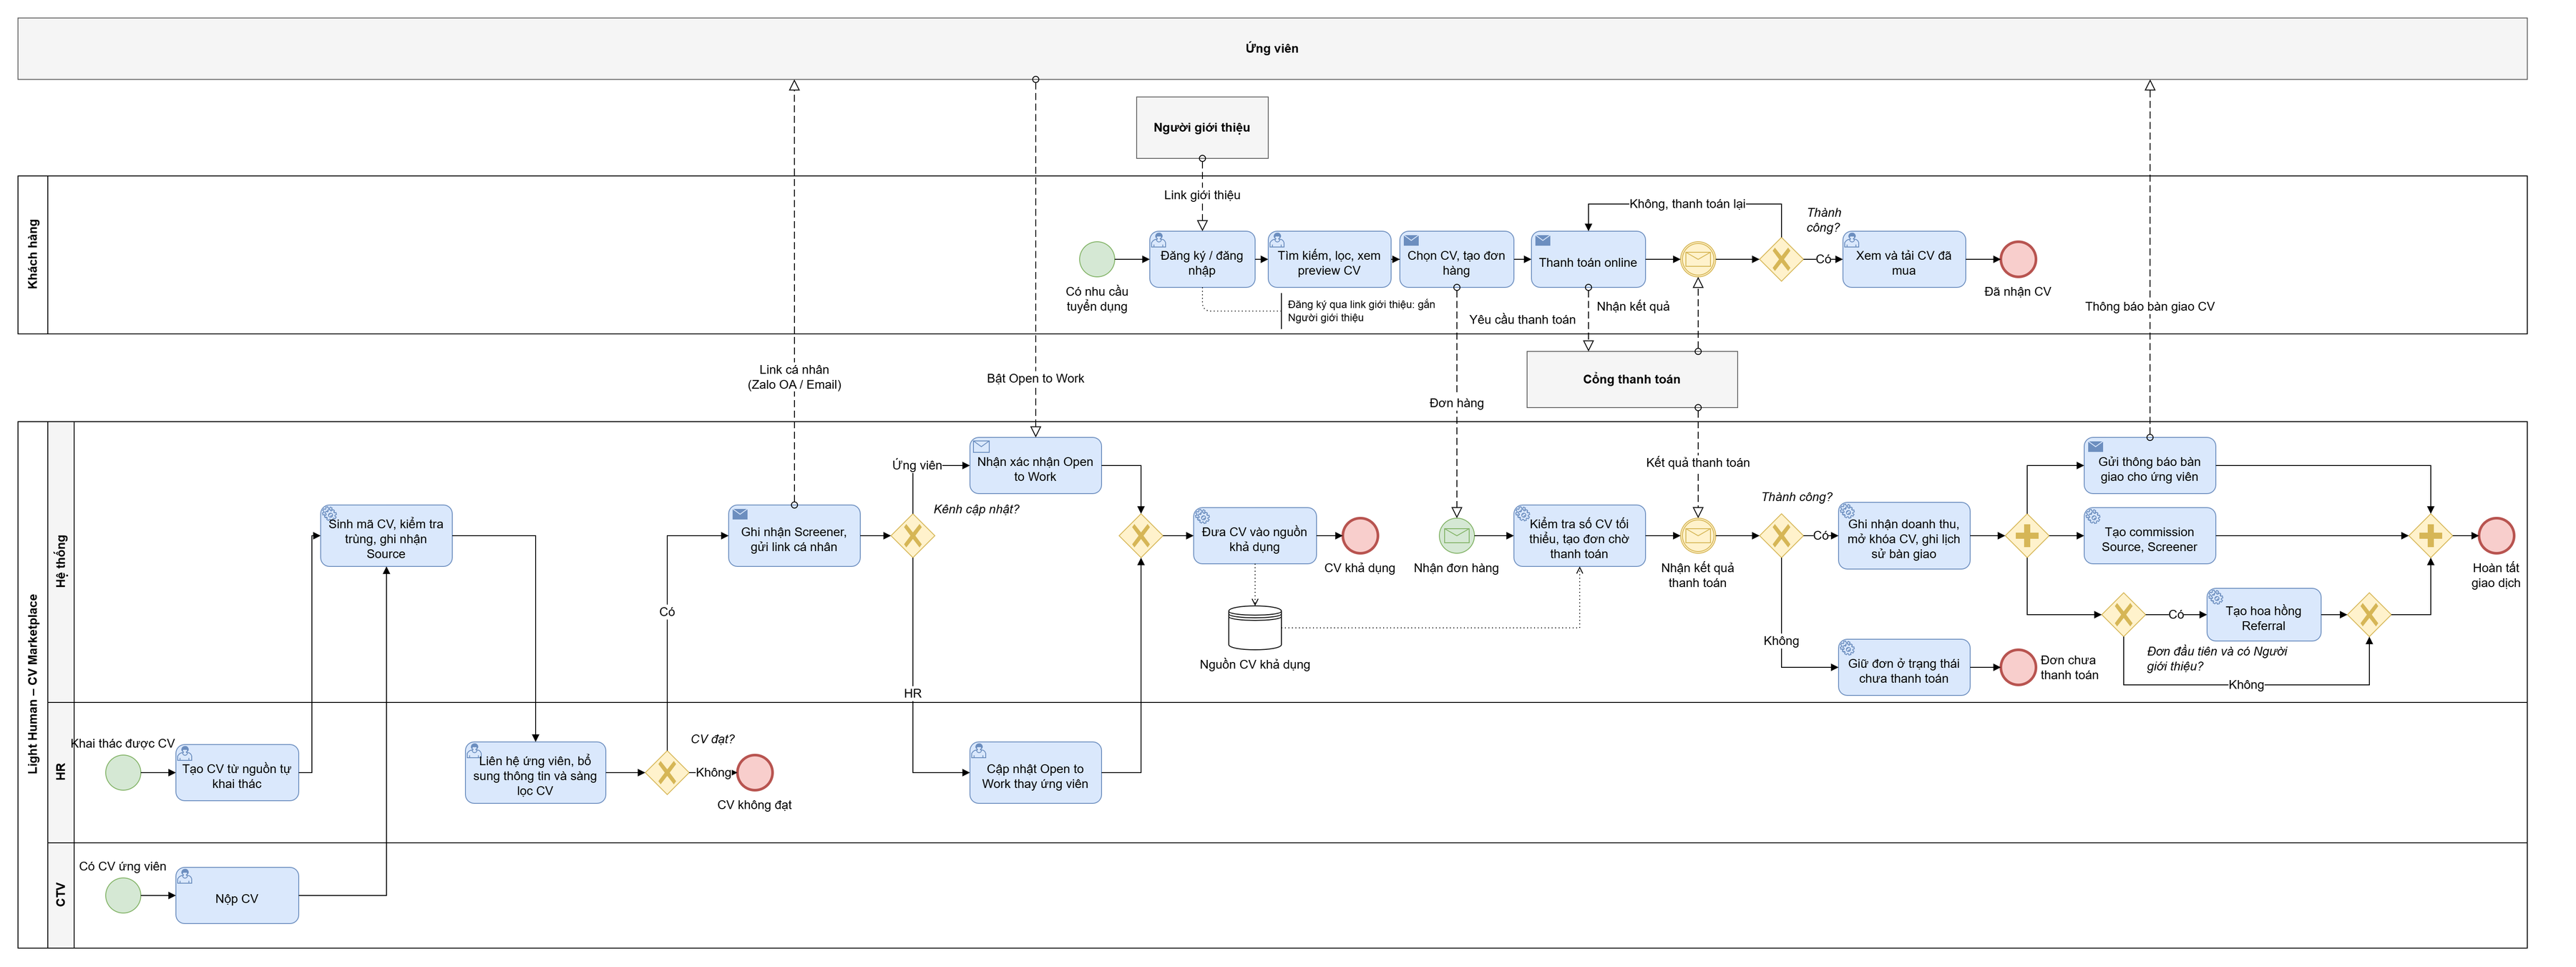
\includegraphics[width=\linewidth]{fig/bpmn.png}
\caption{BPMN TO-BE – quy trình nghiệp vụ tổng quát của CV Marketplace}\label{fig:bpmn}
\end{figure}

\section{Phân tích và thiết kế hệ thống}
\subsection{Yêu cầu và use case}
Đề tài đặc tả 20 yêu cầu chức năng thuộc sáu nhóm và bảy nhóm yêu cầu phi chức năng (hiệu năng, bảo mật, toàn vẹn dữ liệu, tuân thủ pháp lý, tính sẵn sàng, khả năng mở rộng, khả năng sử dụng). Các yêu cầu chức năng được hiện thực qua 15 use case (Hình~\ref{fig:uc}, Bảng~\ref{tab:uc}); mỗi use case có đặc tả gồm tiền điều kiện, hậu điều kiện, luồng chính, luồng thay thế và ngoại lệ, kèm biểu đồ hoạt động và sơ đồ tuần tự.

\begin{figure}[!htbp]
\centering
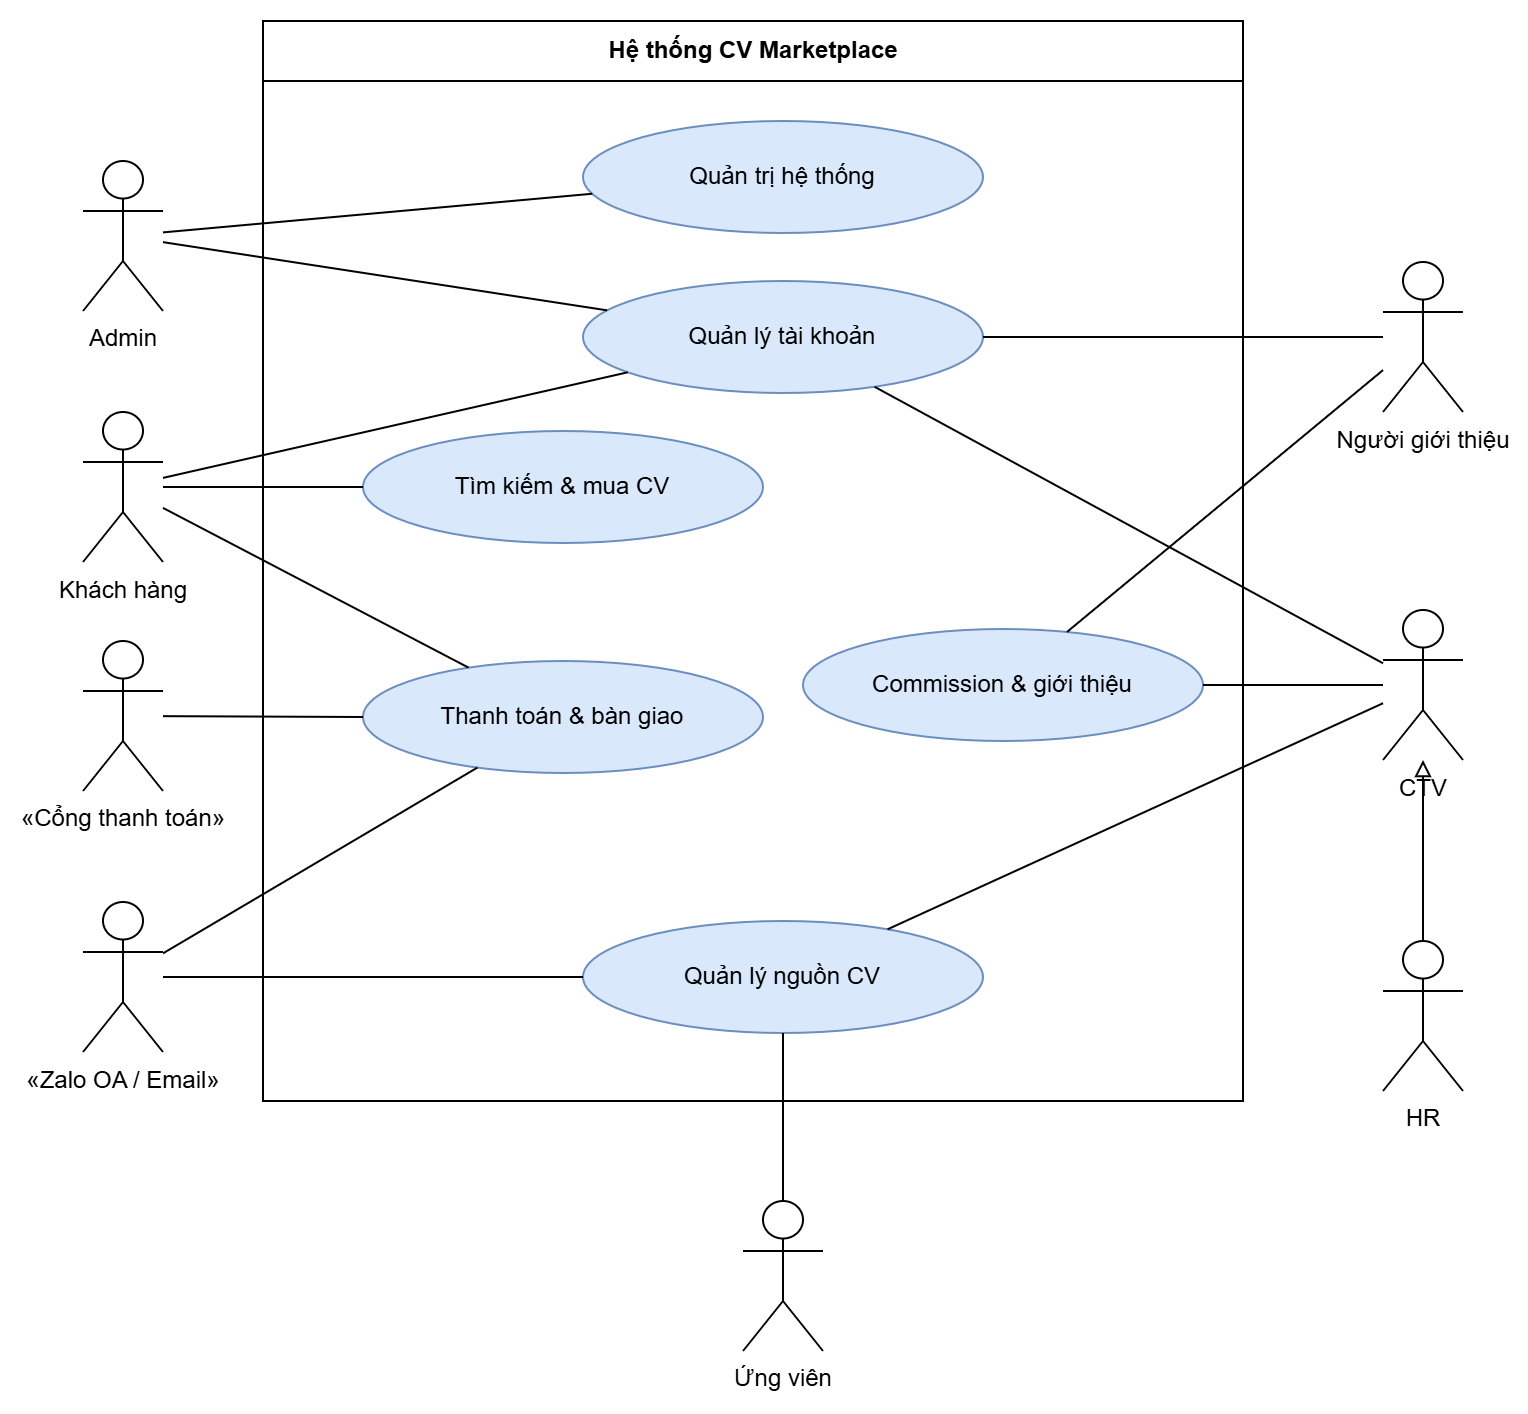
\includegraphics[width=0.5\linewidth]{fig/uc_overview.png}
\caption{Sơ đồ Use Case tổng quan}\label{fig:uc}
\end{figure}

\begin{table}[!htbp]
\centering\small
\caption{Danh sách use case theo nhóm chức năng}\label{tab:uc}
\begin{tabularx}{\linewidth}{@{}p{3.6cm}L@{}}
\toprule
\textbf{Nhóm} & \textbf{Use case}\\\midrule
Quản lý tài khoản & UC01 Đăng ký tài khoản; UC02 Đăng nhập; UC03 Quản lý tài khoản nội bộ\\
Quản lý nguồn CV & UC04 Tạo/Nộp CV; UC05 Sàng lọc CV; UC06 Cập nhật Open to Work\\
Tìm kiếm và mua CV & UC07 Tìm kiếm và xem preview CV; UC08 Tạo đơn hàng; UC09 Xem và tải CV đã sở hữu\\
Thanh toán và bàn giao & UC10 Thanh toán đơn hàng\\
Commission và giới thiệu & UC11 Xem commission cá nhân; UC12 Lấy link giới thiệu và xem khách hàng đã giới thiệu\\
Quản trị hệ thống & UC13 Cấu hình giá bán và tỷ lệ commission; UC14 Điều chỉnh Source/Screener; UC15 Xem báo cáo\\\bottomrule
\end{tabularx}
\end{table}

\subsection{Acceptance criteria}
Mỗi use case có từ 3 đến 4 tiêu chí chấp nhận viết theo cấu trúc Cho – Khi – Thì (Given – When – Then), tổng cộng 53 tiêu chí, bao phủ luồng chính, trường hợp vi phạm business rule và trường hợp sai quyền. Ví dụ:
\begin{itemize}
\item \textbf{AC08.1:} Cho giỏ có ít hơn số CV tối thiểu theo cấu hình, khi tạo đơn hàng, thì hệ thống không cho tạo và báo số CV còn thiếu.
\item \textbf{AC10.3:} Cho hệ thống nhận trùng kết quả của cùng một giao dịch, khi xử lý, thì giao dịch chỉ được xử lý một lần, không tạo trùng bàn giao hay commission.
\item \textbf{AC09.2:} Cho CV khách hàng chưa sở hữu, khi truy cập trực tiếp vào trang chi tiết, thì hệ thống từ chối và không hiển thị thông tin liên hệ.
\end{itemize}

\subsection{Thiết kế dữ liệu và phân quyền}
ERD gồm 13 thực thể (Hình~\ref{fig:erd}). Thiết kế tách bảng Attribution để mỗi CV có hai bản ghi Source và Screener; tách CVTransaction để một CV xuất hiện trong đơn hàng của nhiều khách hàng; Commission gắn với từng dòng giao dịch (Source, Screener) hoặc với đơn hàng đầu tiên của khách hàng (Referral). Từ điển dữ liệu mô tả kiểu, khóa và ràng buộc của từng thuộc tính. Các quy tắc toàn vẹn chính gồm: số điện thoại ứng viên là duy nhất để chống trùng; ràng buộc duy nhất (CVID, Role) trên Attribution; (CustomerID, CVID) trên lịch sử bàn giao để khách hàng không mua lại CV; mã giao dịch của cổng thanh toán là duy nhất để mỗi giao dịch chỉ được xử lý một lần; đơn hàng và commission lưu giá, tỷ lệ tại thời điểm tạo. Ma trận phân quyền xác định chức năng cho năm nhóm có tài khoản; ứng viên chỉ thao tác qua link chứa mã định danh riêng.

\begin{figure}[!htbp]
\centering
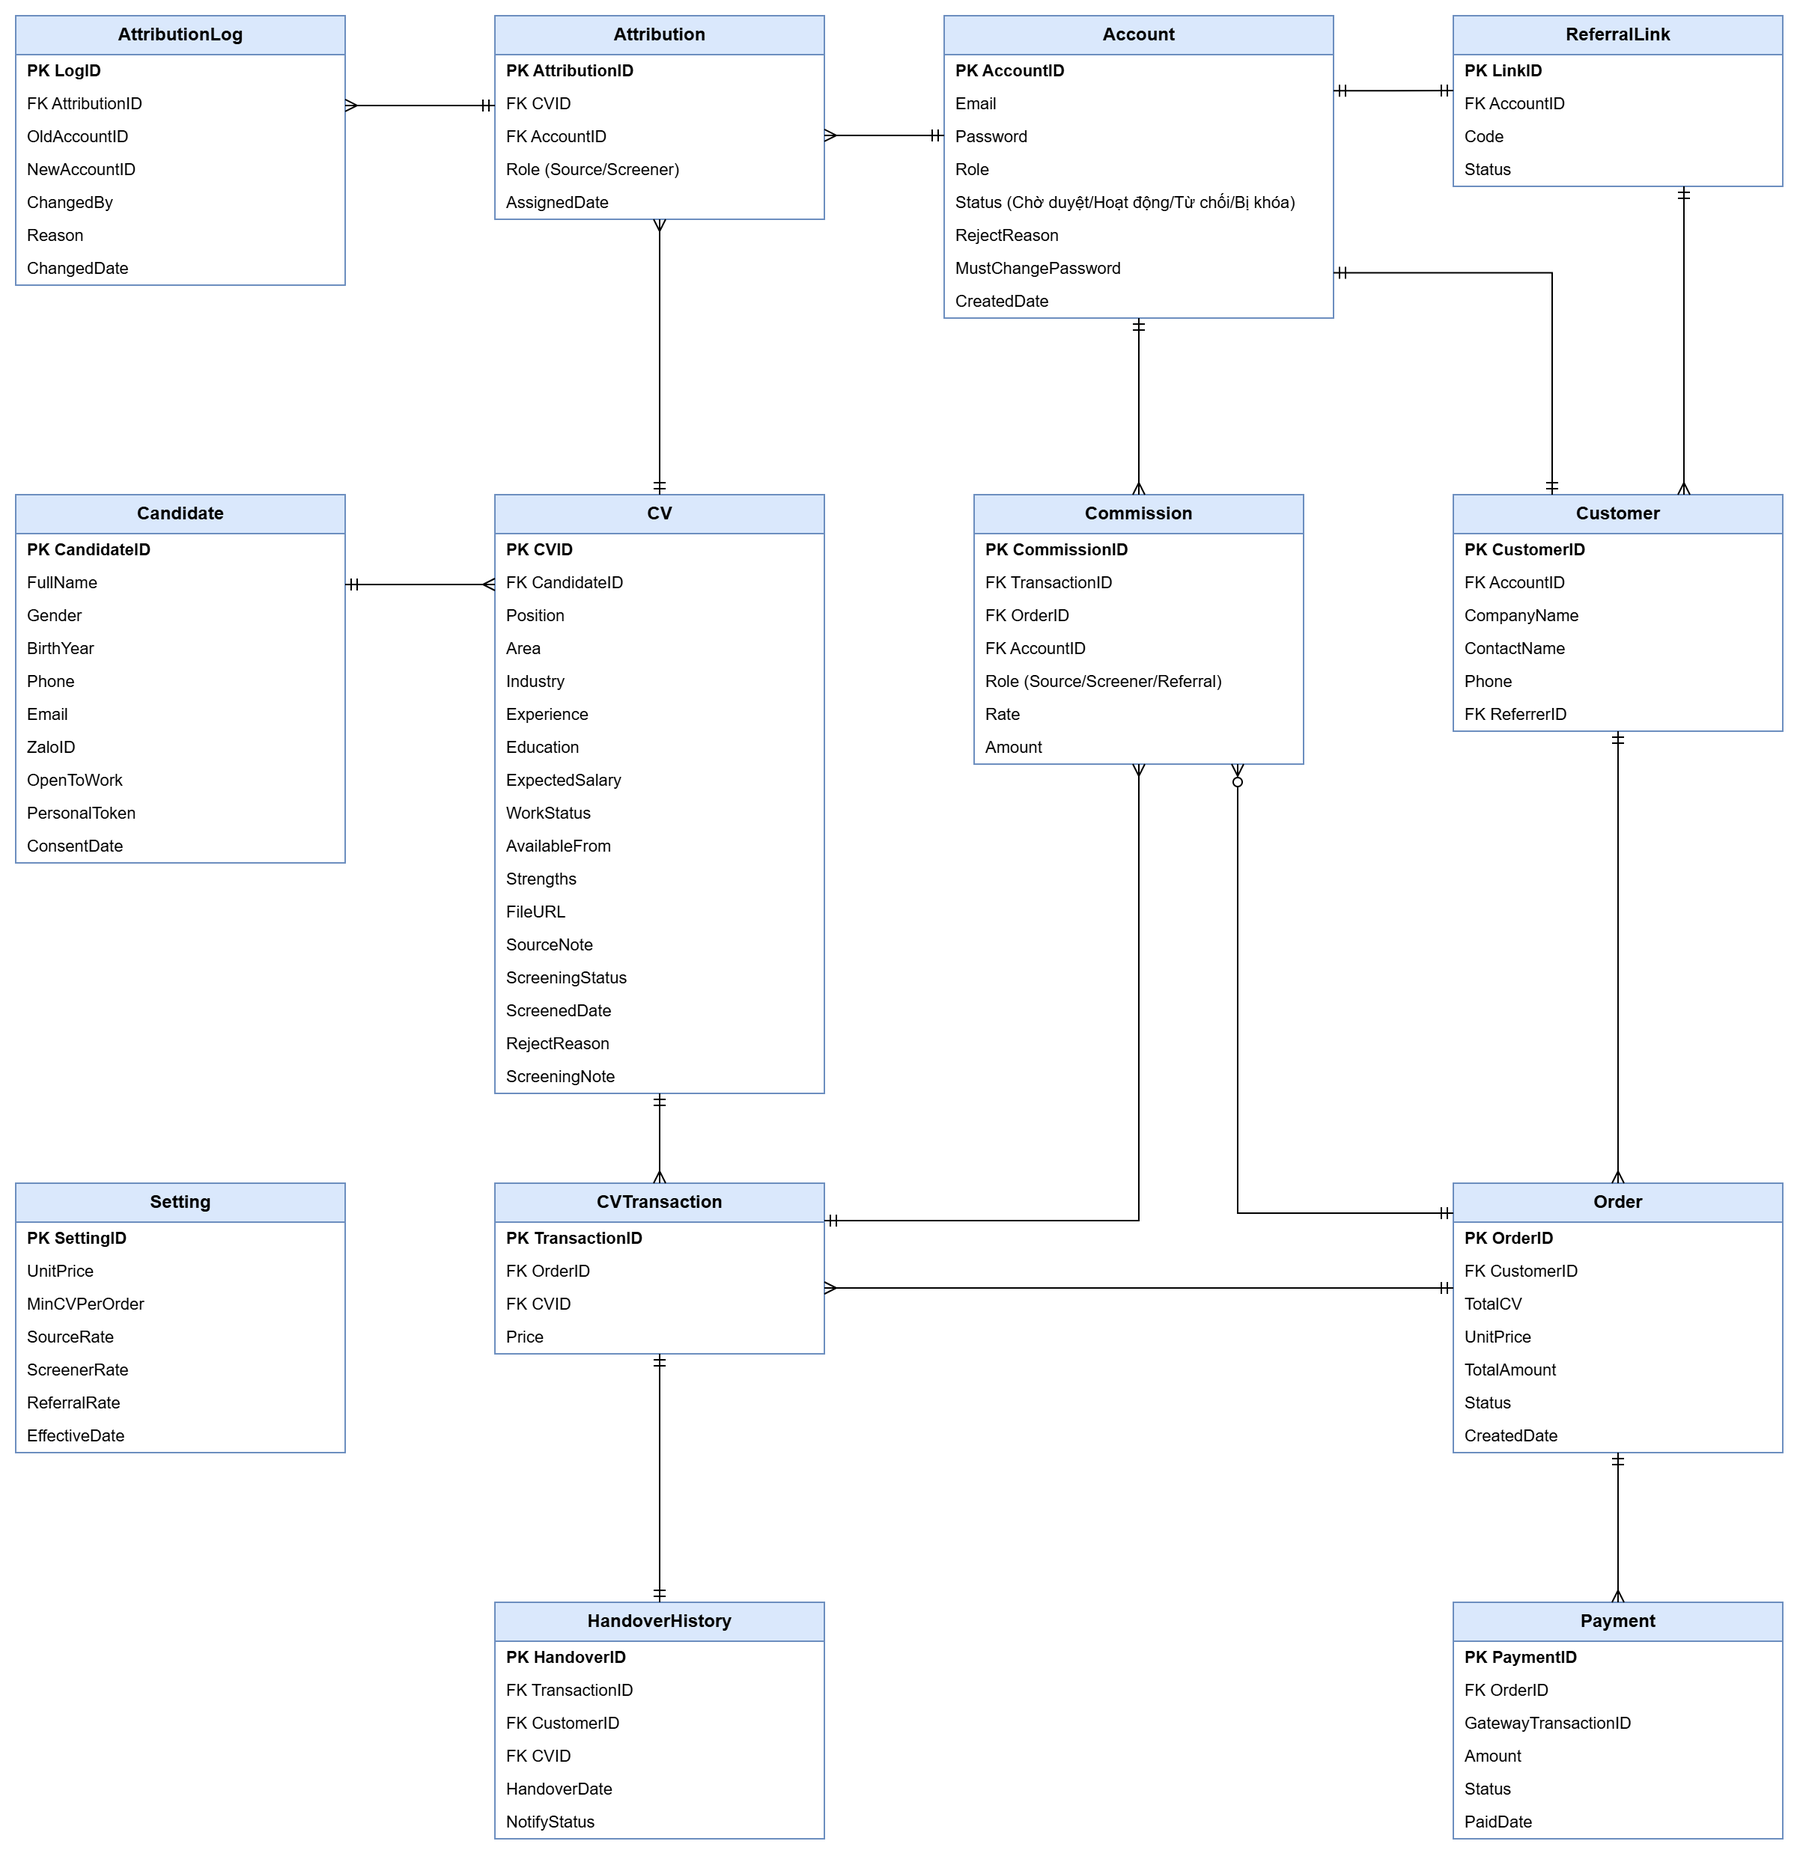
\includegraphics[width=0.62\linewidth]{fig/erd.png}
\caption{Sơ đồ ERD của hệ thống}\label{fig:erd}
\end{figure}

\subsection{Kiến trúc tổng quan}
Kiến trúc được đề xuất ở mức logic theo mô hình ba tầng (Hình~\ref{fig:arch}). Tầng giao diện gồm cổng người dùng, cổng quản trị và trang link cá nhân của ứng viên, giao tiếp với tầng ứng dụng qua HTTPS (REST API, JSON). Tầng ứng dụng gồm sáu module tương ứng sáu nhóm use case; lớp xác thực và phân quyền kiểm tra mọi yêu cầu trước khi xử lý, lớp ghi lịch sử thao tác và gửi thông báo dùng chung. Với luồng thanh toán, kết quả từ cổng thanh toán được xác thực chữ ký và kiểm tra trùng; việc cập nhật đơn hàng, mở khóa CV, ghi bàn giao và tạo commission được thực hiện trong cùng một giao dịch cơ sở dữ liệu. Các thông số môi trường được đặt trong cấu hình, không ghi cứng trong mã nguồn.

\begin{figure}[!htbp]
\centering
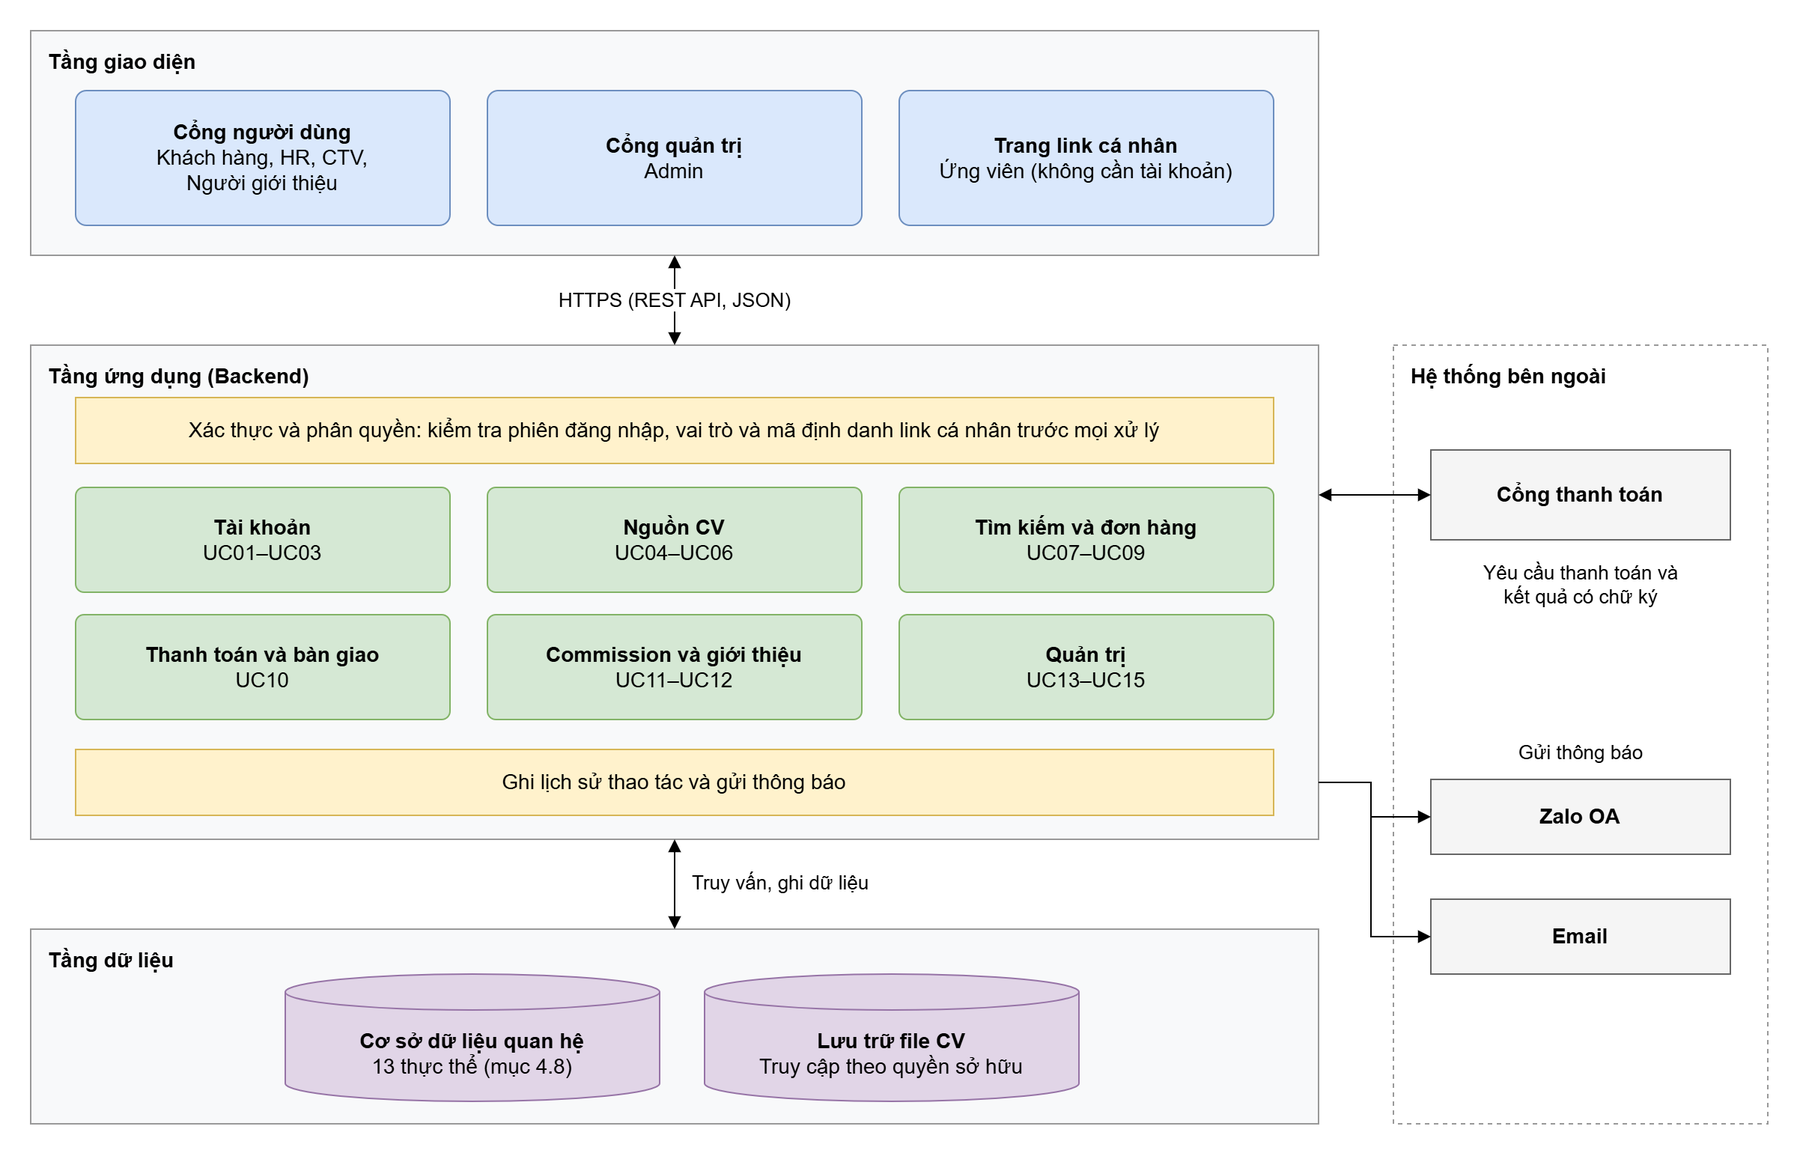
\includegraphics[width=0.85\linewidth]{fig/arch.png}
\caption{Kiến trúc tổng quan hệ thống CV Marketplace}\label{fig:arch}
\end{figure}

\section{Thiết kế giao diện và bản demo}
Giao diện được xây dựng thành bản demo web tương tác gồm 18 màn hình chính cho sáu vai trò, chạy trên dữ liệu mẫu và dùng chung dữ liệu giữa các cổng (Hình~\ref{fig:ui}). Giao diện tuân theo các nguyên tắc khả dụng: hiển thị trạng thái hệ thống, dùng ngôn ngữ nghiệp vụ quen thuộc, xác nhận trước thao tác khó hoàn tác, kiểm tra dữ liệu ngay khi nhập, cung cấp tìm kiếm và bộ lọc trên mọi danh sách. Bản demo trình diễn được luồng end-to-end từ nộp CV đến chia commission, trường hợp vi phạm business rule (đơn dưới 5 CV), trường hợp lỗi thanh toán và phân quyền theo vai trò. Bản demo được công khai tại \url{https://nlinh1703.github.io/Bao-cao-thuc-tap-BA/Code/}.

\begin{figure}[!htbp]
\centering
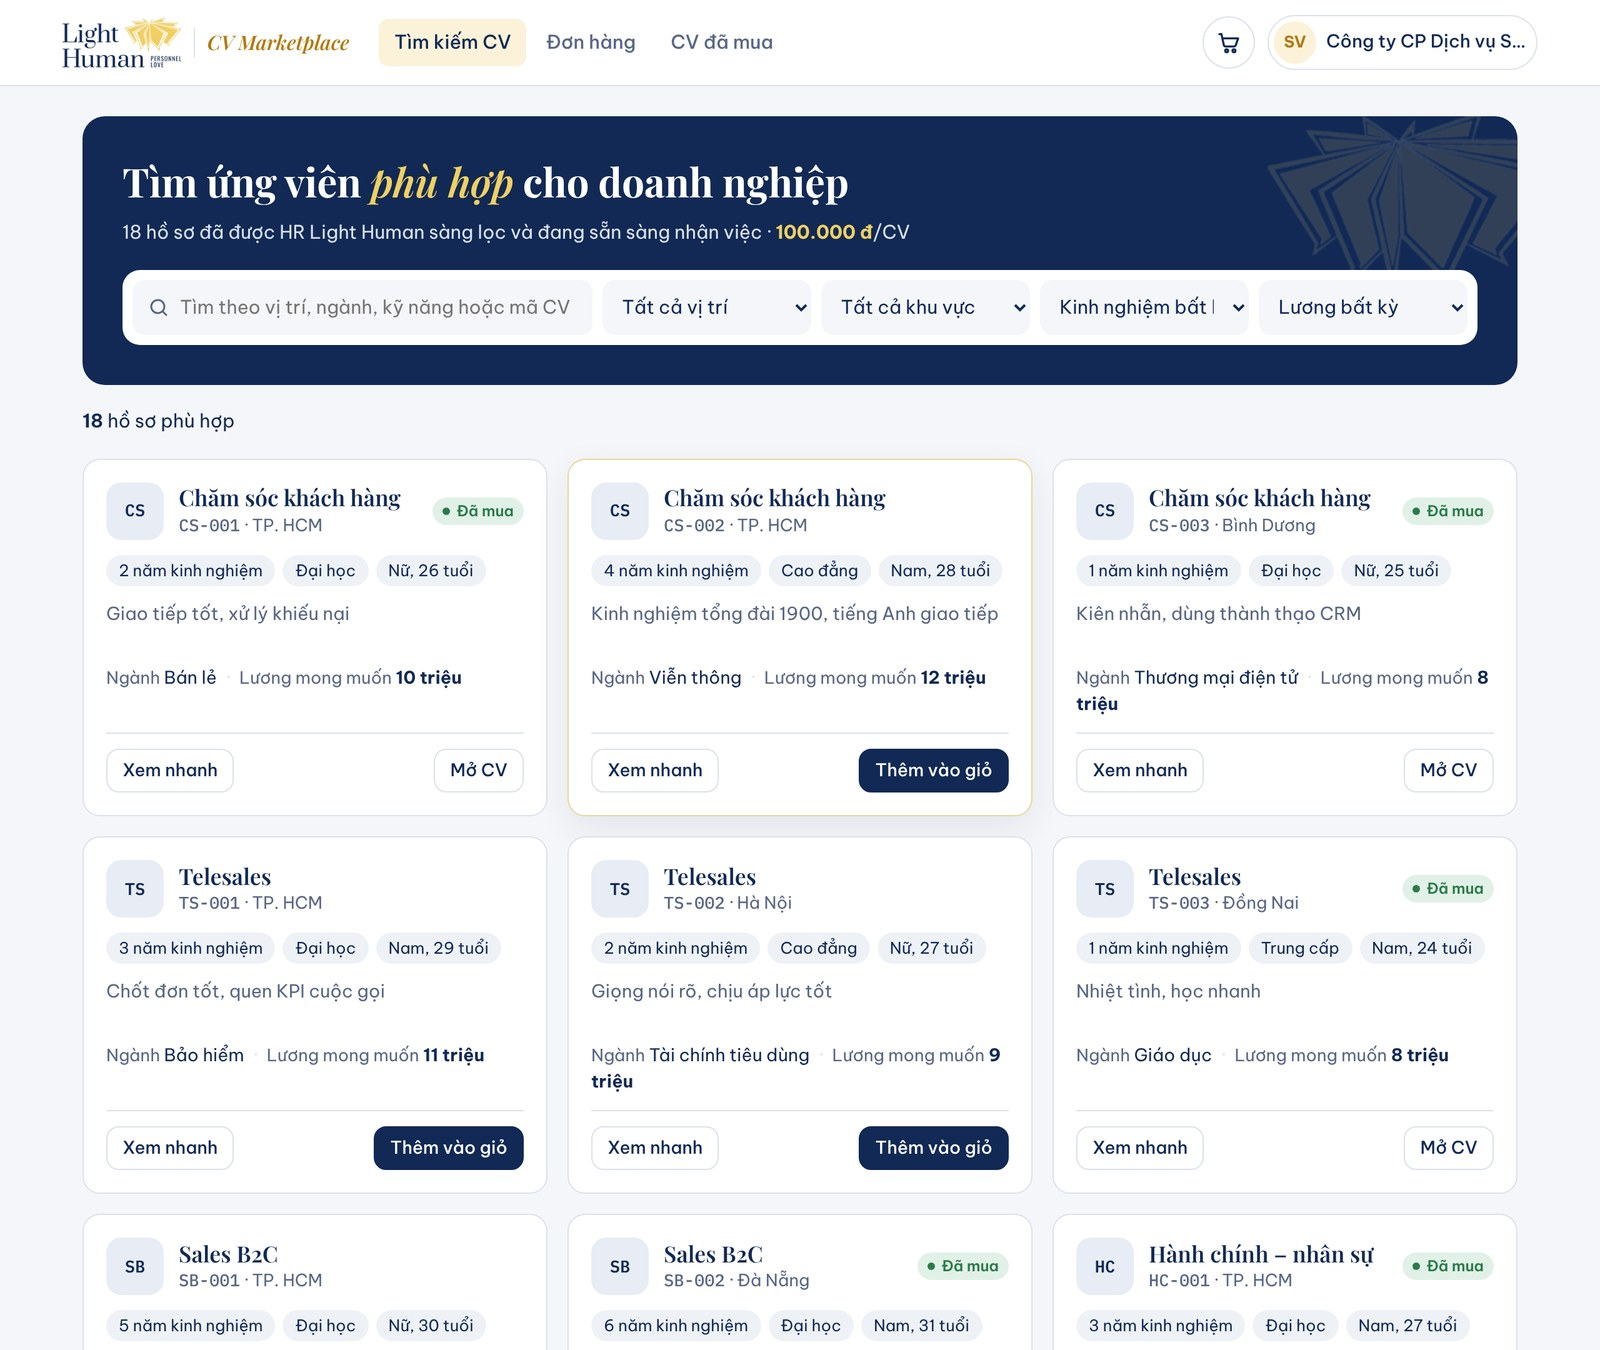
\includegraphics[width=0.49\linewidth]{fig/ui_search.jpg}\hfill
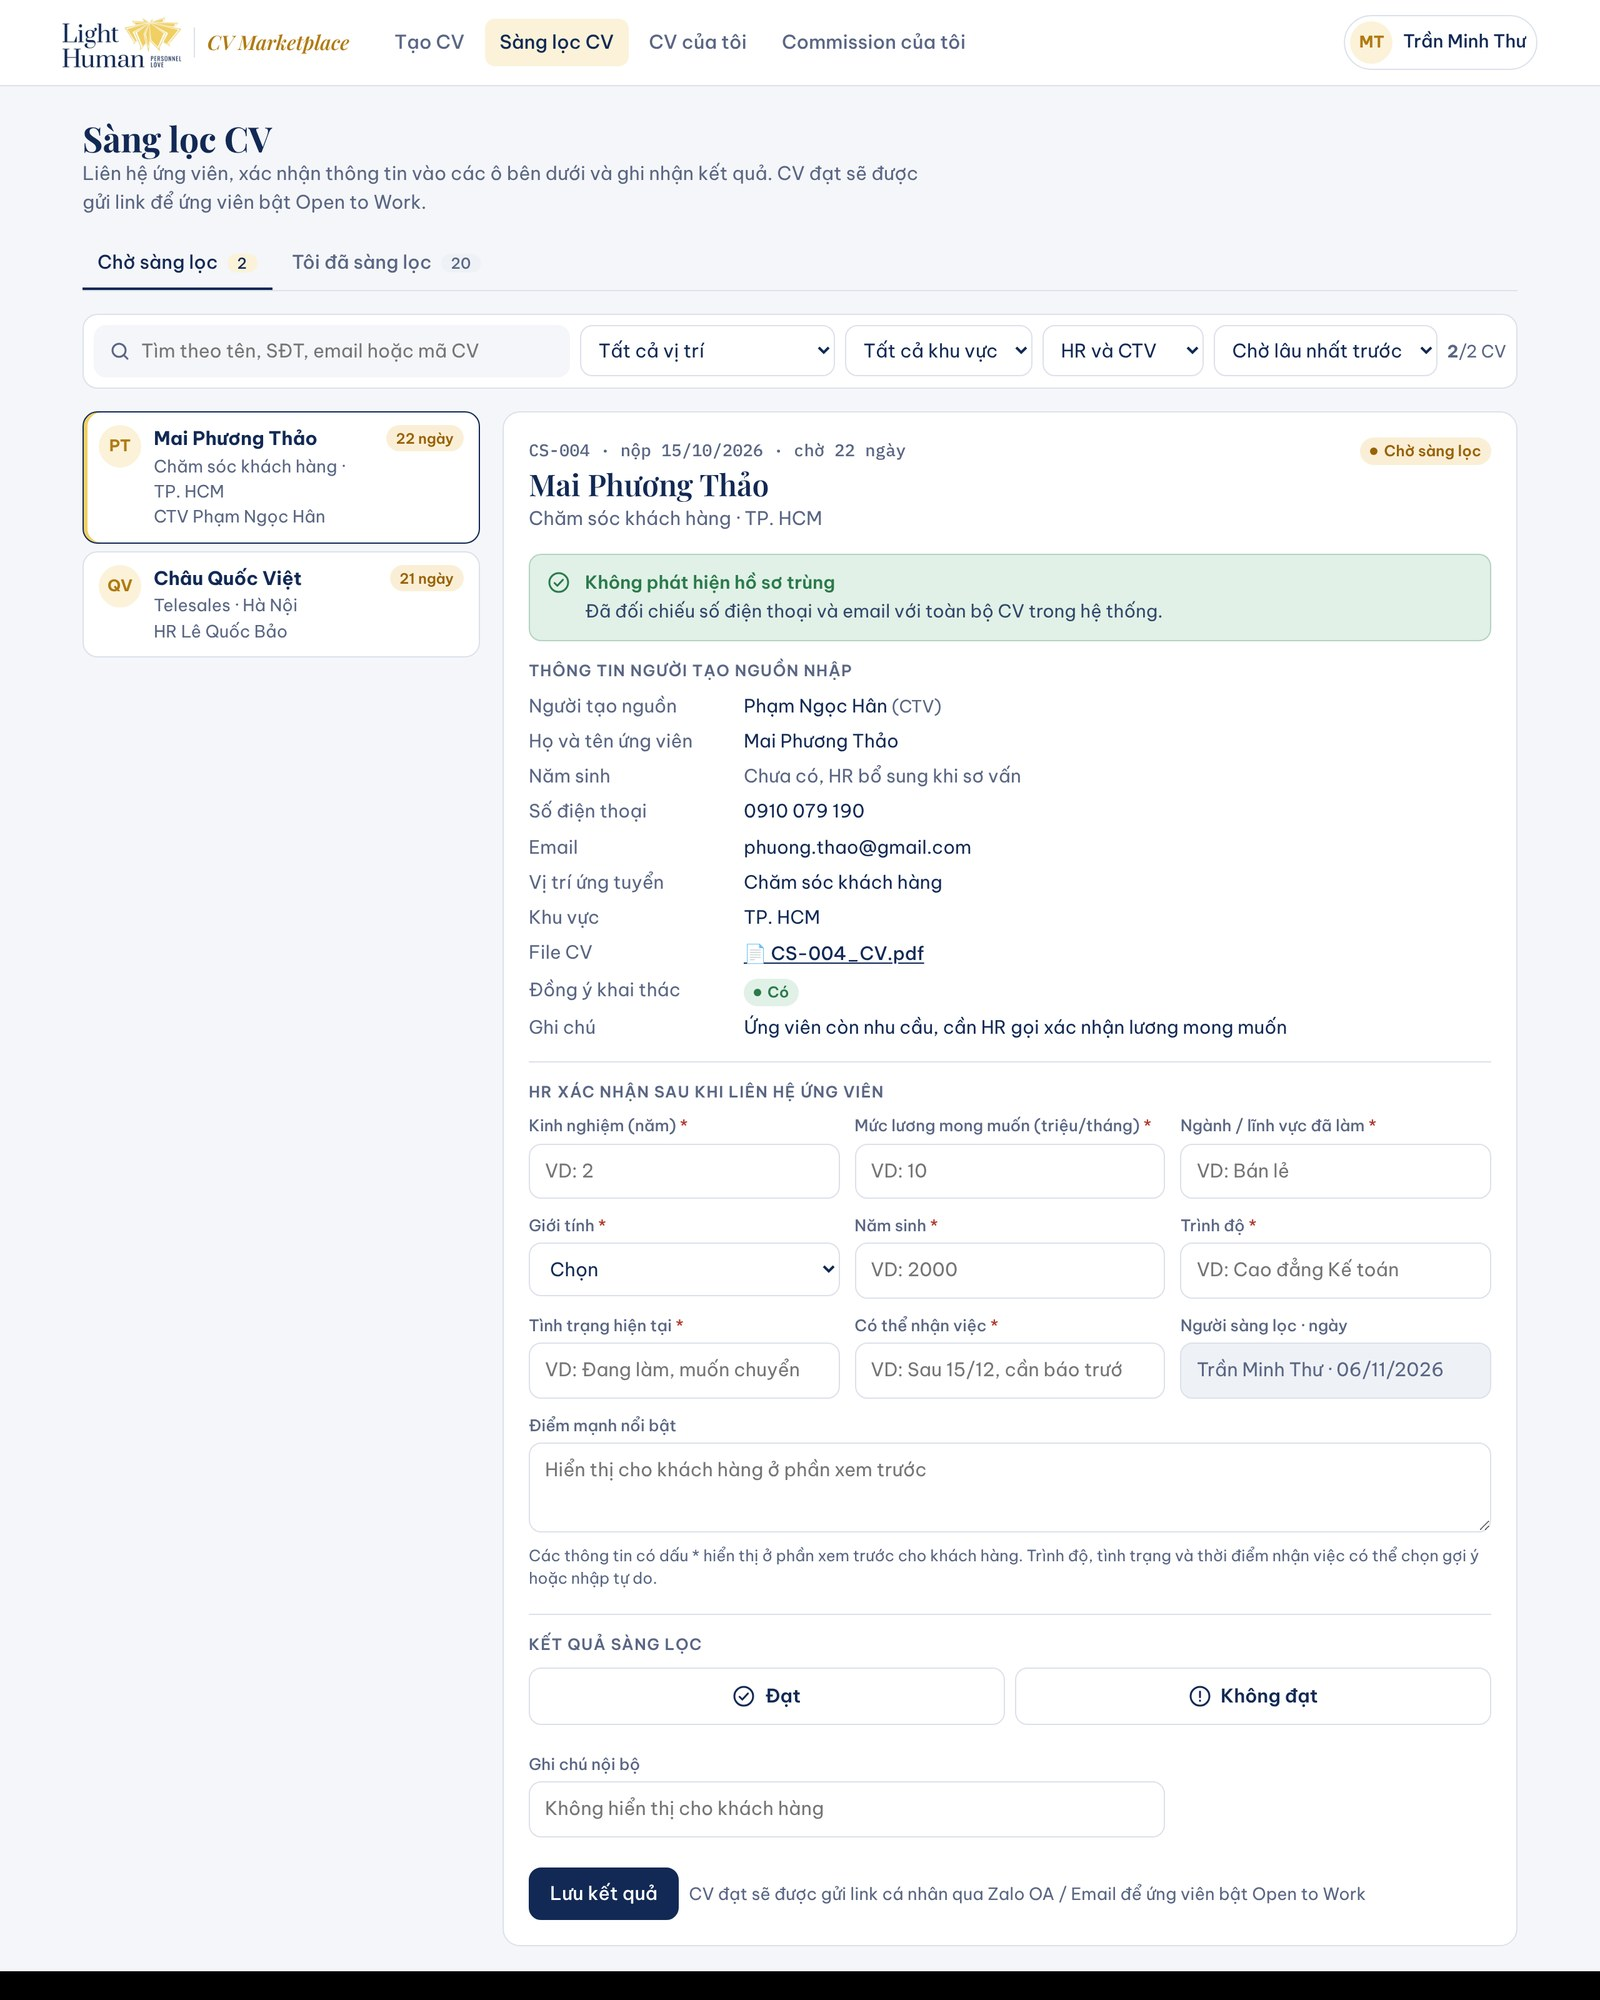
\includegraphics[width=0.49\linewidth]{fig/ui_screen.jpg}
\caption{Màn hình tìm kiếm CV của khách hàng (trái) và màn hình sàng lọc CV của HR (phải)}\label{fig:ui}
\end{figure}

\section{Kết quả và đánh giá}
Đề tài đã hoàn thành bộ tài liệu gồm: phân tích tám bên liên quan; 15 business rules và sơ đồ BPMN TO-BE; 20 yêu cầu chức năng và bảy nhóm yêu cầu phi chức năng; 7 sơ đồ Use Case, 15 đặc tả use case, 15 biểu đồ hoạt động, 15 sơ đồ tuần tự; 53 acceptance criteria; ERD, từ điển dữ liệu cho 13 thực thể và ma trận phân quyền; kiến trúc tổng quan; bản demo giao diện 18 màn hình. Song song, phiên bản chạy thử cùng tài liệu hướng dẫn vận hành đã được bàn giao cho doanh nghiệp. Các sản phẩm được truy vết nhất quán từ yêu cầu chức năng đến use case, sơ đồ, dữ liệu và giao diện, có thể dùng trực tiếp làm đầu vào cho đội phát triển.

Đề tài còn các hạn chế: phiên bản web chính thức chưa được lập trình nên thiết kế chưa được kiểm chứng bằng vận hành thực tế; bản demo chỉ chạy trên dữ liệu giả lập lưu tại trình duyệt, cổng thanh toán được mô phỏng; chưa thiết kế chi trả commission, hoàn tiền, xử lý khiếu nại; thiết kế dữ liệu dừng ở mức logic.

\section{Kết luận và hướng phát triển}
Đề tài đã phân tích và thiết kế hệ thống CV Marketplace, giúp Light Human khai thác thương mại nguồn CV ứng viên sẵn có. Điểm nổi bật là cơ chế ghi nhận đóng góp theo từng vai trò Source, Screener, Referral để chia commission tự động, và cơ chế Open to Work qua link cá nhân giúp ứng viên chủ động với dữ liệu của mình. Hướng phát triển tiếp theo gồm: kiểm thử bản demo với người dùng thực tế; thiết kế cơ sở dữ liệu mức vật lý và đặc tả API; lập kế hoạch chuyển dữ liệu từ giai đoạn chạy thử; xây dựng kịch bản kiểm thử chấp nhận; bổ sung bảng giá theo loại nguồn CV, chi trả commission tự động và gợi ý CV phù hợp cho khách hàng.

\begin{thebibliography}{10}\small
\bibitem{nd13} Chính phủ (2023), \emph{Nghị định số 13/2023/NĐ-CP ngày 17/04/2023 về bảo vệ dữ liệu cá nhân}.
\bibitem{lh_admin} Công ty Cổ phần Giải pháp Nhân sự Ánh Sáng (2026), \emph{Hướng dẫn sử dụng hệ thống CV Marketplace – Dành cho Admin}, tài liệu nội bộ.
\bibitem{lh_kh} Công ty Cổ phần Giải pháp Nhân sự Ánh Sáng (2026), \emph{Quy trình làm việc với khách hàng – CV Marketplace}, tài liệu nội bộ.
\bibitem{lh_tkcs} Công ty Cổ phần Giải pháp Nhân sự Ánh Sáng (2026), \emph{Thiết kế cơ sở hệ thống CV Marketplace}, tài liệu nội bộ.
\bibitem{topcv} MISA AMIS (không ghi năm), “Tìm hiểu trang tuyển dụng TopCV”, \url{https://amis.misa.vn/86359/tim-hieu-trang-tuyen-dung-top-cv/}.
\bibitem{vnw} MISA AMIS (2023), “VietNamWorks là gì? Tìm hiểu trang tuyển dụng VietnamWorks”, \url{https://amis.misa.vn/86407/tim-hieu-trang-tuyen-dung-vietnamworks/}.
\bibitem{babok} International Institute of Business Analysis (2015), \emph{A Guide to the Business Analysis Body of Knowledge (BABOK Guide)}, Version 3, IIBA, Toronto.
\bibitem{bpmn} Object Management Group (2014), \emph{Business Process Model and Notation (BPMN)}, Version 2.0.2.
\bibitem{uml} Object Management Group (2017), \emph{OMG Unified Modeling Language (OMG UML)}, Version 2.5.1.
\bibitem{bmc} Osterwalder, A. \& Pigneur, Y. (2010), \emph{Business Model Generation}, John Wiley \& Sons.
\end{thebibliography}
\end{document}
